\subsection{Annahmen zur Modellierung (T.B.)}
Das Koordinatensystem des Flügels entspricht dem Flugzeugkoordinatensystem, sodass die \\Flügellängskoordinate durch $y$ definiert ist. Der Koordinatenursprung ist im Lager A positioniert. \\

\noindent Der Holm inkl. des Holmstummels wird für die Belastung durch eine Prüfkraft $F_{pruef}$ in negative z-Richtung als Biegebalken ausgelegt. Dafür ist er an zwei Stellen gelagert, dem Lager $A$ und Lager $B$, dabei repräsentieren sie die Verstiftungen (siehe Bauteil "U-Profil"). Um eine Überbestimmung des Systems zu vermeiden, wird das Lager $B$ als Loslager angenommen. Die Querkraftbolzen werden nicht durch ein Lager, sondern durch eine zusätzlich angreifende Kraft $F_{Q}$ simuliert, da keine Absenkung, sondern lediglich eine Kraftaufnahme der Wurzelrippen möglich ist. \\

\noindent Als Randbedingungen der Modellierung sind die Halbspannweite $s$ und die Absenkung $w$ gegeben. Für die Absenkung $w$ soll eine Sicherheit $j=1,1$ gesetzt werden. Zwischen Lager $A$ und $B$ wird die Länge $l_{1}$ angenommen, zwischen Lager $B$ und der Wurzelrippe $C$ die Länge $l_{2}$. Die verbleibende Länge bis zur Flügelspitze, an der die Prüfkraft $F_{pruef}$ wirkt, wird $l_{3}$ bezeichnet. Die Halbspannweite $s$ wird beginnend in der Mitte der Verstiftungen bis zur Flügelspitze gemessen. Das Holmstummelende wird ab dem Lager $A$ mit $l_{0}$ als Länge definiert. Diese Länge ist jedoch unerheblich für die Modellierung, sondern wird erst für die Massenbestimmung benötigt.\\

\noindent Anhand der Randbedingungen und der Einspannvorrichtung für den Versuchsaufbau ergeben sich folgende Längen (ebenfalls in Abb. ~\ref{fig:Holmmodellierung}~ dargestellt): 
\begin{equation}
	s = 0,848 m
\end{equation}
\begin{equation}
	l_{0} = 0,03 m
\end{equation}
\begin{equation}
	l_{1} = 0,076 m
\end{equation}
\begin{equation}
	l_{2} = 0,037 m 
\end{equation}
\begin{equation}
	l_{3} = s - \frac{l_{1}}{2} - l_{2} = 0,773 m
\end{equation}
\begin{equation}
	w_{j=1,1} = \frac{1}{j} * w = \frac{1}{1,1} * 0,022 m = 0,02 m
\end{equation}
\begin{figure}
	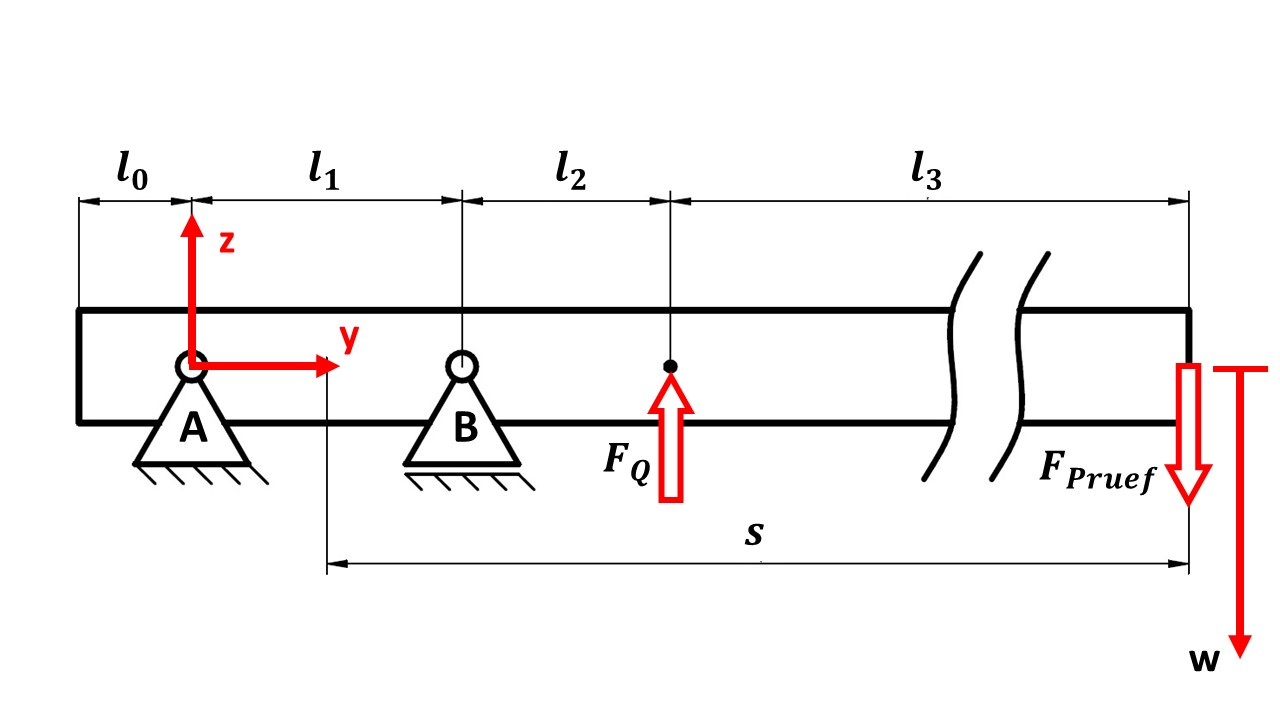
\includegraphics[width=1.0\textwidth]{Bilder/Balkenmodell.jpg}
	\caption{Modellierung des Holms}
	\label{fig:Holmmodellierung}
\end{figure}

\subsection{Analytische Lösung der Modellierung (T.B.)}
Um die der Differentialgleichungen der Balkenbiegung lösen zu können, wird das System vorerst in drei Teilbereiche $I$, $II$, und $III$ aufgeteilt, die sich von Lager $A$ nach $B$, von Lager $B$ zur Wurzelrippe $C$ und von dort us bis zur Flügelspitze. \\

\noindent Dadurch ergeben sich folgende zwölf Differentialgleichungen:
\begin{equation}
	EI\cdot w_{I}^{''''}(y) = q_{I}(y)
\end{equation}
\begin{equation}
	EI\cdot w_{I}^{'''}(y) = q_{I}(y)\cdot y + R_{1} = -Q_{I}(y)
\end{equation}
\begin{equation}
	EI\cdot w_{I}^{''}(y) = \frac{q_{I}(y)}{2}\cdot y^{2} + R_{1}\cdot y + R_{2} = -M_{I}(y)
\end{equation}
\begin{equation}
	EI\cdot w_{I}^{'}(y) = \frac{q_{I}(y)}{6}\cdot y^{3} + \frac{R_{1}}{2}\cdot y^{2} + R_{2}\cdot y + R_{3} 
\end{equation}
\begin{equation}
	EI\cdot w_{I}(y) = \frac{q_{I}(y)}{24}\cdot y^{4} + \frac{R_{1}}{6}\cdot y^{3} + \frac{R_{3}}{2}\cdot y^{2} + R_{3}\cdot y + R_{4}
\end{equation}\\
\begin{equation}
	EI\cdot w_{II}^{''''}(y) = q_{II}(y)
\end{equation}
\begin{equation}
	EI\cdot w_{II}^{'''}(y) = q_{II}(y)\cdot y + R_{5} = -Q_{II}(y)
\end{equation}
\begin{equation}
	EI\cdot w_{II}^{''}(y) = \frac{q_{II}(y)}{2}\cdot y^{2} + R_{5}\cdot y + R_{6} = -M_{II}(y)
\end{equation}
\begin{equation}
	EI\cdot w_{II}^{'}(y) = \frac{q_{II}(y)}{6}\cdot y^{3} + \frac{R_{5}}{2}\cdot y^{2} + R_{6}\cdot y + R_{7} 
\end{equation}
\begin{equation}
	EI\cdot w_{II}(y) = \frac{q_{II}(y)}{24}\cdot y^{4} + \frac{R_{5}}{6}\cdot y^{3} + \frac{R_{6}}{2}\cdot y^{2} + R_{7}\cdot y + R_{8}
\end{equation}\\
\begin{equation}
EI\cdot w_{III}^{''''}(y) = q_{III}(y)
\end{equation}
\begin{equation}
EI\cdot w_{III}^{'''}(y) = q_{III}(y)\cdot y + R_{9} = -Q_{I}(y)
\end{equation}
\begin{equation}
EI\cdot w_{III}^{''}(y) = \frac{q_{III}(y)}{2}\cdot y^{2} + R_{9}\cdot y + R_{10} = -M_{I}(y)
\end{equation}
\begin{equation}
EI\cdot w_{IIII}^{'}(y) = \frac{q_{III}(y)}{6}\cdot y^{3} + \frac{R_{9}}{2}\cdot y^{2} + R_{10}\cdot y + R_{11} 
\end{equation}
\begin{equation}
EI\cdot w_{III}(y) = \frac{q_{III}(y)}{24}\cdot y^{4} + \frac{R_{9}}{6}\cdot y^{10} + \frac{R_{3}}{2}\cdot y^{2} + R_{11}\cdot y + R_{12}
\end{equation}\\

\noindent Die Randbedingungen der Modellierung ergeben sich folgend: 
\begin{equation}
	w_{I}(l=0)=0
\end{equation}
\begin{equation}
	M_{I}(l=0)=0
\end{equation}\\
\begin{equation}
	w_{I}(l=l{1}) = 0
\end{equation}
\begin{equation}
	w_{II}(l=l{1}) = 0
\end{equation}
\begin{equation}
	w_{I}^{'}(l=l{1}) = w_{II}^{'}(l=l{1})
\end{equation}
\begin{equation}
	M_{I}(l=l{1}) = M_{II}(l=l{1})
\end{equation}\\
\begin{equation}
	w_{II}(l=l{1}+l_{2}) = w_{III}(l=l{1}+l_{2})
\end{equation}
\begin{equation}
	w_{II}^{'}(l=l{1}+l_{2}) = w_{III}^{'}(l=l{1}+l_{2})
\end{equation}
\begin{equation}
	M_{II}(l=l{1}+l_{2}) = M_{III}(l=l{1}+l_{2})
\end{equation}
\begin{equation}
	Q_{II}(l=l{1}+l_{2}) = Q_{III}(l=l{1}+l_{2})+F_{Q}
\end{equation}\\
\begin{equation}
	M_{III}(l=l_{1}+l_{2}+l_{3})=0
\end{equation}
\begin{equation}
	Q_{III}(l=l_{1}+l_{2}+l_{3})=F
\end{equation}
Zusätzlich wird angenommen, dass $q_{I}(y)=q_{II}(y)=q_{III}(y)=0$ gilt, da keine Streckenlast angreift.\\

\noindent Als Lösung dieser Differentialgleichungen lässt sich die Querkraft $Q(y)$, das Moment $M(y)$ und die Biegelinie $w(y)$ ermitteln:\\

\begin{equation}
	Q(y,F,F_{Q},EI)=\left\{\begin{array}{ll}
		F\cdot \frac{l_{2}+l_{3}}{l_{1}}-F_{Q}\cdot \frac{l_{2}}{l_{1}}&,y\epsilon (0,l_{1})\\
		F+F_{Q}&,y\epsilon (l_{1}+l{2})\\
		F&,y\epsilon (l_{1}+l{2}+l{3})
	\end{array}\right.
\end{equation}\\
\begin{equation}
	M(y,F,F_{Q},EI)=\left\{\begin{array}{ll}
		(-F\cdot \frac{l_{2}+l_{3}}{l_{1}}-F_{Q}\cdot \frac{l_{2}}{l_{1}})\cdot y&,y\epsilon (0,l_{1})\\
		(F+F_{Q})\cdot y - F\cdot (l_{1}+l_{2}+l_{3})-F_{Q}\cdot (l_{1}+L_{2})&,y\epsilon (l_{1}+l{2})\\
		F\cdot y - F\cdot (l_{1}+l_{2}+l_{3})&,y\epsilon (l_{1}+l{2}+l{3})
	\end{array}\right.
\end{equation}\\
\begin{equation}
	w(y,F,F_{Q},EI)=\left\{\begin{array}{ll}
		\frac{1}{EI}\cdot\frac{1}{6}\cdot\biggl(F\cdot \frac{l_{2}+l_{3}}{l_{1}}-F_{Q}\cdot \frac{l_{2}}{l_{1}})\cdot y^{3}-\Bigl((l_{2}+l_{3})\cdot l_{1}\cdot F-l_{1}\cdot l_{2}\cdot F_{Q}\Bigl)\cdot y \biggr)&\\,y\epsilon (0,l_{1})\\
		\frac{1}{EI}\cdot\biggl(\frac{(-F-F_{Q})}{6}\cdot y^{3} + \frac{F\cdot (l_{1}+l_{2}+l_{3})+F_{Q}\cdot (l_{1}+L_{2})}{2}\cdot y^{2}\\ + \Bigl(F\cdot(-\frac{1}{2}\cdot l_{1}^{2}-\frac{2}{3}\cdot l_{1}\cdot l_{2}-\frac{2}{3}\cdot l_{1}\cdot l_{3})+ F_{Q}\cdot(-\frac{1}{2}l_{1}^{2}-\frac{2}{3}\cdot l_{1}\cdot l_{2})\Bigr)\cdot y \\+ F\cdot\frac{1}{6}\cdot(l_{1}^{3}+l_{1}^{2}\cdot l_{2}+l_{1}^{2}\cdot l_{3}) + F_{Q}\cdot\frac{1}{6}\cdot(l_{1}^{3}+l_{1}^{2}\cdot l_{2})\biggr)&\\,y\epsilon (l_{1}+l{2})\\
		\frac{1}{EI}\cdot\biggl(-\frac{F}{6}\cdot y^{3} + \frac{ F\cdot (l_{1}+l_{2}+l_{3})}{2}\cdot y^{2} + \Bigl(F\cdot(-\frac{1}{2}\cdot l_{1}^{2} -\frac{2}{3}\cdot l_{1}\cdot l_{2}-\frac{2}{3}\cdot l_{1}\cdot l_{3})\\ + F_{Q}\cdot(\frac{1}{2}\cdot l_{2}^{2}+\frac{1}{2}\cdot l_{1}\cdot l_{2})\Bigr)\cdot y +F\cdot\frac{1}{6}\cdot(l_{1}^{3}+l_{1}^{2}\cdot l_{2}+l_{1}^{2}\cdot l_{3}) + \\F_{Q}\cdot(-\frac{1}{6}\cdot l_{2}^{3}-\frac{1}{3}\cdot l_{1}^{2}\cdot l_{2}-\frac{1}{2}\cdot l_{2}^{2}\cdot l_{1})\biggr)&\\,y\epsilon (l_{1}+l{2}+l{3})
	\end{array}\right.
\end{equation}\\
Die Herleitung der Lösung ist dem Anhang beigefügt.

\subsection{Ermittlung der Biegesteifigkeit}
Um nun für die Biegesteifigeit $EI$ ein Ergebnis zu erhalten, wird die Gleichung $w(y,F,F_{Q})$ nach $EI(y,F,F_{Q},w)$ umgestellt. Die eingesetzten Werte ergeben sich aus der Auslegung auf Steifigkeit. Über die Wurzelrippe werden Kräfte des Holms in die Querkraftbolzen abgesetzt. Aufgrund der biegeweichen Wurzelrippe darf die Absenkung des Holms dort nicht mit Null angenommen werden. Vereinfacht wird definiert, dass die eingeleitete Prüfkraft $F_{pruef}$ an den Querkraftbolzen um ihren Betrag abgesetzt wird, wie es tatsächlich an einem Flugzeugrumpf geschehen würde. 

\begin{equation}
	\begin{array}{l}
		EI(0.961m, 100N, -100N, 0.022m)= \\
		\frac{1}{w}\cdot\biggl(-\frac{F}{6}\cdot y^{3} + \frac{ F\cdot (l_{1}+l_{2}+l_{3})}{2}\cdot y^{2} + \Bigl(F\cdot(-\frac{1}{2}\cdot l_{1}^{2} -\frac{2}{3}\cdot l_{1}\cdot l_{2}-\frac{2}{3}\cdot l_{1}\cdot l_{3}) +		F_{Q}\cdot(\frac{1}{2}\cdot l_{2}^{2}+\frac{1}{2}\cdot l_{1}\cdot l_{2})\Bigr)\cdot y +\\
		F\cdot\frac{1}{6}\cdot(l_{1}^{3}+l_{1}^{2}\cdot l_{2}+l_{1}^{2}\cdot l_{3}) + F_{Q}\cdot(-\frac{1}{6}\cdot l_{2}^{3}-\frac{1}{3}\cdot l_{1}^{2}\cdot l_{2}-\frac{1}{2}\cdot l_{2}^{2}\cdot l_{1})\biggr)\\
		=3,102631\cdot10^{-8}m^{4}
	\end{array}
\end{equation}


